% Options for packages loaded elsewhere
\PassOptionsToPackage{unicode}{hyperref}
\PassOptionsToPackage{hyphens}{url}
%
\documentclass[
  12pt,
]{article}
\usepackage{amsmath,amssymb}
\usepackage{lmodern}
\usepackage{ifxetex,ifluatex}
\ifnum 0\ifxetex 1\fi\ifluatex 1\fi=0 % if pdftex
  \usepackage[T1]{fontenc}
  \usepackage[utf8]{inputenc}
  \usepackage{textcomp} % provide euro and other symbols
\else % if luatex or xetex
  \usepackage{unicode-math}
  \defaultfontfeatures{Scale=MatchLowercase}
  \defaultfontfeatures[\rmfamily]{Ligatures=TeX,Scale=1}
\fi
% Use upquote if available, for straight quotes in verbatim environments
\IfFileExists{upquote.sty}{\usepackage{upquote}}{}
\IfFileExists{microtype.sty}{% use microtype if available
  \usepackage[]{microtype}
  \UseMicrotypeSet[protrusion]{basicmath} % disable protrusion for tt fonts
}{}
\makeatletter
\@ifundefined{KOMAClassName}{% if non-KOMA class
  \IfFileExists{parskip.sty}{%
    \usepackage{parskip}
  }{% else
    \setlength{\parindent}{0pt}
    \setlength{\parskip}{6pt plus 2pt minus 1pt}}
}{% if KOMA class
  \KOMAoptions{parskip=half}}
\makeatother
\usepackage{xcolor}
\IfFileExists{xurl.sty}{\usepackage{xurl}}{} % add URL line breaks if available
\IfFileExists{bookmark.sty}{\usepackage{bookmark}}{\usepackage{hyperref}}
\hypersetup{
  pdftitle={Détection de fraudes et loi de probabilité de Newcomb-Benford},
  pdfauthor={FERNANDEZ Christelle; PONCHEELE Clément; EL KAÏM Laura; Encadré par M.DUCHARME},
  hidelinks,
  pdfcreator={LaTeX via pandoc}}
\urlstyle{same} % disable monospaced font for URLs
\usepackage[margin=1in]{geometry}
\usepackage{graphicx}
\makeatletter
\def\maxwidth{\ifdim\Gin@nat@width>\linewidth\linewidth\else\Gin@nat@width\fi}
\def\maxheight{\ifdim\Gin@nat@height>\textheight\textheight\else\Gin@nat@height\fi}
\makeatother
% Scale images if necessary, so that they will not overflow the page
% margins by default, and it is still possible to overwrite the defaults
% using explicit options in \includegraphics[width, height, ...]{}
\setkeys{Gin}{width=\maxwidth,height=\maxheight,keepaspectratio}
% Set default figure placement to htbp
\makeatletter
\def\fps@figure{htbp}
\makeatother
\setlength{\emergencystretch}{3em} % prevent overfull lines
\providecommand{\tightlist}{%
  \setlength{\itemsep}{0pt}\setlength{\parskip}{0pt}}
\setcounter{secnumdepth}{-\maxdimen} % remove section numbering
\oddsidemargin -1cm
\textwidth 18,5cm
\textheight 24cm
\usepackage[french]{babel}
\usepackage[tableposition=top]{caption}
\captionsetup{labelformat=empty}
\usepackage{caption}
\captionsetup{position=below}
\usepackage{booktabs}
\usepackage{longtable}
\usepackage{array}
\usepackage{multirow}
\usepackage{wrapfig}
\usepackage{float}
\usepackage{colortbl}
\usepackage{pdflscape}
\usepackage{tabu}
\usepackage{threeparttable}
\usepackage{threeparttablex}
\usepackage[normalem]{ulem}
\usepackage{makecell}
\usepackage{xcolor}
\ifluatex
  \usepackage{selnolig}  % disable illegal ligatures
\fi

\title{Détection de fraudes et loi de probabilité de Newcomb-Benford}
\author{FERNANDEZ Christelle \and PONCHEELE Clément \and EL KAÏM
Laura \and Encadré par M.DUCHARME}
\date{\emph{\(5\) mars \(2021\)}}

\begin{document}
\maketitle

RESUME DU PROJET EN QLQ LIGNES

REMERCIEMENTS

\maketitle
\tableofcontents

\newpage

\hypertarget{introduction.}{%
\section{Introduction.}\label{introduction.}}

~ La fraude est une pratique répandue dans de nombreux domaines comme
par exemple la finance, le secteur social ou médical. Il peut être
tentant pour un être humain ou une société de tricher si cela peut
impliquer pour lui une position plus confortable dans la société, telle
qu'une réduction de charges, ou même un avantage sur un de ses
concurrents. Il semblerait donc logique que des personnes cherchent à
déceler ces fraudes.

Les données transmises par un individu ou un organisme peuvent faire
l'objet de modifications, c'est de ce type de fraudes auquel nous nous
intéresserons ici, et plus particulièrement la modification du premier
chiffre significatif (le premier chiffre d"un nombre qui n'est pas un
zéro) de nombres pris dans un certain ensemble de données.

De telles modifications entraînent un changement de la répartition des
chiffres présents naturellement\footnote{Les données dites naturelles
  sont celles qui n'ont pas été influencé par la pensée de l'homme.}. Si
nous connaissons la répartition des chiffres présentés dans un ensemble
de données arbitraires, il est donc techniquement possible de savoir si
un nombre a été modifié ou non.

Il nous vient donc les questions suivantes: \emph{Qu'elle est cette
répartition ? Est-il possible de la connaître et si oui, dans quels cas
?}

De manière intuitive nous pourrions penser que les nombres sont répartis
de manière uniforme. Qu'en est-il vraiment ?

La première partie de notre projet consistera à \textbf{répondre à ces
questions}, nous nous appuierons sur les travaux de Simon Newcomb et
Frank Benford, qui ont théorisé la \textbf{loi de Newcomb-Benford}, plus
communément appelée loi de Benford. Cette loi nous dit que, dans une
liste de données dites naturelles, la probabilité d'avoir le chiffre
\(i\) comme premier chiffre significatif est de
\(log_{10}(1 + \frac{1}{i})\).

Par exemple, le chiffre \(1\) en tant que premier chiffre significatif
serait présent à hauteur de \(30\%\) alors que le \(9\) à seulement
\(4,6\%\).

Dans la suite \textbf{nous mettrons en œuvre une série
d'expérimentation} pour constater ou non la véracité de cette loi, pour
ce faire dans un premier temps nous récolterons des nombres pris dans
des milieux sensés satisfaire la loi de Newcomb-Benford et observerons
la répartition du premier chiffre significatif. Puis nous répliquerons
une version simplifiée de l'expérience de Hill (1988), qui consiste à
observer la répartition du premier chiffre significatif d'une liste de
nombre donnée au hasard par des êtres humains, en l'occurrence ses
élèves.

Cette expérience est à la base des méthodes de détection de fraudes par
la loi de Newcomb-Benford. Si un fraudeur modifie un jeu de données, ce
jeu est donc influencé par la pensée humaine, il ne suit donc plus la
loi de Newcomb-Benford. Pour détecter la fraude il suffit donc de
comparer les premiers chiffres significatifs. Cependant ces comparaisons
doivent se faire de manière rigoureuses et scientifiques. Pour cela il
existe des test statistiques, dont le plus connu, le test du \(\chi^2\),
ou bien celui de Ducharme et collab. (2020).

Il nous vient donc les questions suivantes: \emph{Ces tests sont-ils
fiables ? Existe-t-il un test significativement meilleur que les autres
? Vont-ils dans le même sens ? Et sinon que faire ?}

La réponse à ces question constituera donc la deuxième partie de ce
projet, pour ce faire nous mettrons en œuvre différents tests sur des
jeux de données comme la fiscalité italienne.

\newpage

\hypertarget{naissance-de-la-loi-de-newcomb-benford.}{%
\section{Naissance de la loi de
Newcomb-Benford.}\label{naissance-de-la-loi-de-newcomb-benford.}}

~ Il serait tentant de penser que les nombres sont répartis de manière
uniforme, cela viendrait du biais d'équiprobabilité\footnote{Défini en
  1985 par Marie-Paule Lecoutre
  (\href{https://fr.wikipedia.org/wiki/Biais_d\%27\%C3\%A9quiprobabilit\%C3\%A9}{\emph{source}}).}.
Ce dernier consiste à ``penser qu'en l'absence d'information, tous les
cas ont la même probabilité de se produire et que le hasard implique
nécessairement l'uniformité''.

Néanmoins cette hypothèse sera contredite une première fois par
l'astronome, mathématicien, économiste et statisticien canadien Simon
Newcomb. Ce dernier fournira en \(1881\) une première approche au
principe statistique, qui se fera injustement appeler \emph{Loi de
Benford}. Celui-ci remarquera que les premières pages des tables
logarithmiques sont plus utilisées que les pages suivantes. Il publiera
sa découverte dans un article de l'\emph{``American Journal of
Mathematics''}.

Cette découverte mise de côté pendant plusieurs années, ce n'est qu'en
\(1938\) que l'ingénieur et physicien américain Frank Benford arrivera
au même résultat après avoir répertorié des dizaines de milliers de
données. Celui-ci pensera être le premier à l'initiative de cette loi,
et c'est pour cette raison que la \emph{loi de Newcomb-Benford} se fera
plus généralement appelée \emph{loi de Benford}.

Cette loi nous dit que, dans une liste de données arbitraires, la
probabilité d'avoir le chiffre \(i\) comme premier chiffre significatif
est de \(log_{10}(1 + \frac{1}{i})\).

\vspace{0.7cm}

\begin{tabu} to \linewidth {>{}l>{\centering}X>{\centering}X>{\centering}X>{\centering}X>{\centering}X>{\centering}X>{\centering}X>{\centering}X>{\centering}X}
\toprule
\textbf{\cellcolor{gray!6}{PCS}} & \cellcolor{gray!6}{1} & \cellcolor{gray!6}{2} & \cellcolor{gray!6}{3} & \cellcolor{gray!6}{4} & \cellcolor{gray!6}{5} & \cellcolor{gray!6}{6} & \cellcolor{gray!6}{7} & \cellcolor{gray!6}{8} & \cellcolor{gray!6}{9}\\
\textbf{Benford} & 0.301 & 0.176 & 0.125 & 0.097 & 0.079 & 0.067 & 0.058 & 0.051 & 0.046\\
\bottomrule
\multicolumn{10}{l}{\textsuperscript{} }\\
\multicolumn{10}{l}{\textsuperscript{} Tableau 1 : Répartition du premier chiffre significatif selon la loi de Newcomb-Benford.}\\
\end{tabu}

\vspace{0.7cm}

Nous retrouvons cette loi dans énormément de domaines comme les
mathématiques, l'environnement, la finance, la physique, etc, plus
précisément sur des données telles que la longueur des fleuves, la
population des villes dans un pays, des déclarations de revenus, etc.\\
Notons cependant qu'il existe des cas où les données ne suivent pas
cette loi, notamment des données dites non naturelles qui seraient
influencé par la pensée humaine (nombres premiers, nombres générés par
des humains, etc).

\newpage

\hypertarget{expuxe9rimentation-sur-diffuxe9rents-jeux-de-donnuxe9es.}{%
\section{Expérimentation sur différents jeux de
données.}\label{expuxe9rimentation-sur-diffuxe9rents-jeux-de-donnuxe9es.}}

~ Après avoir pris connaissance de la \textbf{loi de Newcomb-Benford},
il serait intéressant de la mettre en pratique sur différents jeux de
données.

\hypertarget{la-suite-de-fibonacci.}{%
\subsection{La suite de Fibonacci.}\label{la-suite-de-fibonacci.}}

~ Intéressons-nous dans un premier temps à la suite de Fibonacci.

Cette suite est une suite d'entiers dans laquelle chaque terme est la
somme des deux termes qui le précèdent. Sa formulation est la suivante :
\[F_{0} = 0, \, F_{1} = 1, \, \text{et} \, \forall \, n \ge 2, \, F_n = F_{n - 1} + F_{n - 2}.\]

Nous commençons par recueillir les \(1000\) premiers termes de la suite
de Fibonacci, pour extraire le premier chiffre significatif de chacun de
ces nombres.

Par la suite nous calculons la répartition de chaque chiffre
significatif et obtenons l'histogramme suivant :

\begin{figure}
\centering
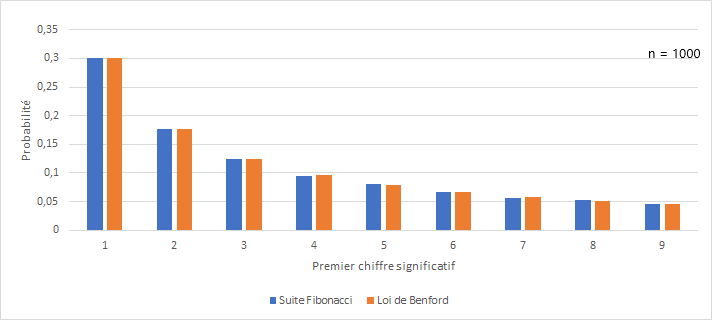
\includegraphics{Images/histogramme_Fibonacci.png}
\caption{Figure 1 : Histrogramme de la répartition du 1er chiffre
significatif de la suite de Fibonacci en comparaison avec la loi de
Benford.}
\end{figure}

Il semblerait que la répartition des chiffres significatifs des \(300\)
premiers nombres de la suite de Fibonacci suive la \textbf{loi de
Newcomb-Benford}.

\newpage

\hypertarget{nombres-extraits-dun-magazine-et-dun-journal.}{%
\subsection{Nombres extraits d'un magazine et d'un
journal.}\label{nombres-extraits-dun-magazine-et-dun-journal.}}

~ Dans un second temps, nous relevons les prix présents dans un magazine
de mobilier de la marque \emph{AMPM}, ainsi que tous les nombres
répertoriés dans un journal \emph{Les ECHOS}. Nous récoltons environ
\(300\) nombres par magazine et, de la même façon qu'énoncé
précédemment, calculons la répartition des chiffres significatifs de ces
nombres.

\begin{figure}
\centering
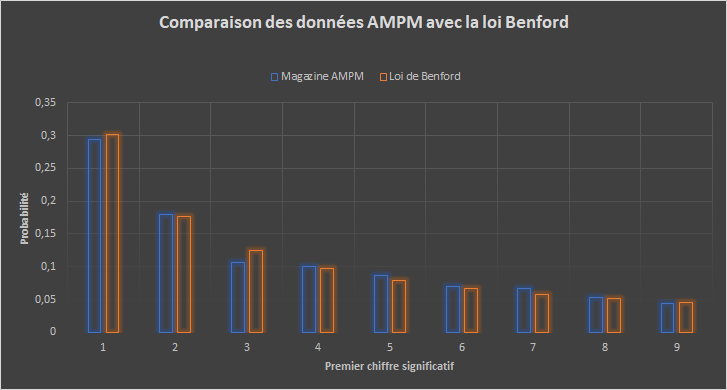
\includegraphics{Images/histogramme_AMPM.png}
\caption{Figure 2 : Histrogramme de la répartition du 1er chiffre
significatif des prix du magazine AMPM en comparaison avec la loi de
Benford.}
\end{figure}

La répartition des chiffres significatifs des prix du magazine
\emph{AMPM} parait fortement similaire à celle de la \textbf{loi de
Newcomb-Benford}. Nous constatons tout de même une légère différence
pour le chiffre \(3\).

Observons maintenant la répartition des données issues du journal
\emph{Les ECHOS}.

\begin{figure}
\centering
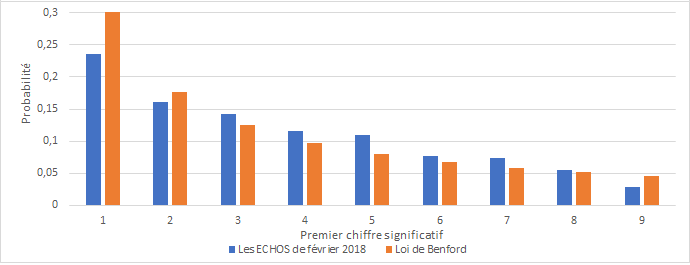
\includegraphics{Images/histogramme_journalLESECHOS.png}
\caption{Figure 3 : Histrogramme de la répartition du 1er chiffre
significatif des nombres du journal LES ECHOS en comparaison avec la loi
de Benford.}
\end{figure}

Nous remarquons ici la même tendance décroissante. Cependant les
proportions des chiffres significatifs entre les données du journal et
celles de la \textbf{loi de Newcomb-Benford} sont relativement
différentes.

\hypertarget{population-des-villes-de-france.}{%
\subsection{Population des villes de
France.}\label{population-des-villes-de-france.}}

~ Dans ce paragraphe nous nous intéressons à la population des villes
françaises. À l'aide des données de l'\emph{INSEE}, nous répertorions
environ \(35000\) premiers chiffres significatifs et regardons leur
répartition.

\begin{figure}
\centering
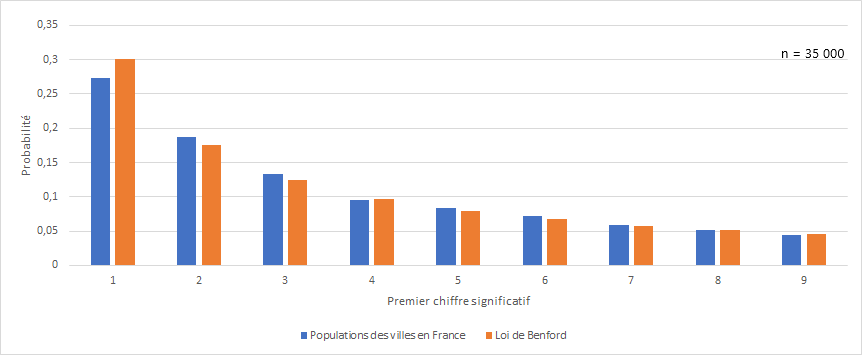
\includegraphics{Images/histogramme_populationfrancaise.png}
\caption{Figure 4 : Histrogramme de la répartition du 1er chiffre
significatif de la population française en comparaison avec la loi de
Benford.}
\end{figure}

Ici les répartitions sont fortement ressemblantes, c'est aussi le cas
pour de nombreuses données démographiques naturelles. Nous aurions pu
également analyser les codes postaux, la longueur des rivières ou encore
la distance des villes de France à Paris.

\newpage

\hypertarget{passage-journalier-de-vuxe9los-dans-lalluxe9e-beracasa-uxe0-montpellier.}{%
\subsection{Passage journalier de vélos dans l'allée Beracasa à
Montpellier.}\label{passage-journalier-de-vuxe9los-dans-lalluxe9e-beracasa-uxe0-montpellier.}}

~ La ville de Montpellier étant en pleine transition écologique, elle
ouvre de plus en plus l'accès aux vélos sur ces routes. Pour en mesurer
l'impact, elle a mit en place des éco-compteurs dans plusieurs rues. Les
données issues de ces compteurs sont en libre accès, nous nous sommes
donc intéressés au nombre de passages journaliers de vélos dans l'allée
Beracasa sur une année.

Nous obtenons la répartition suivante :

\begin{figure}
\centering
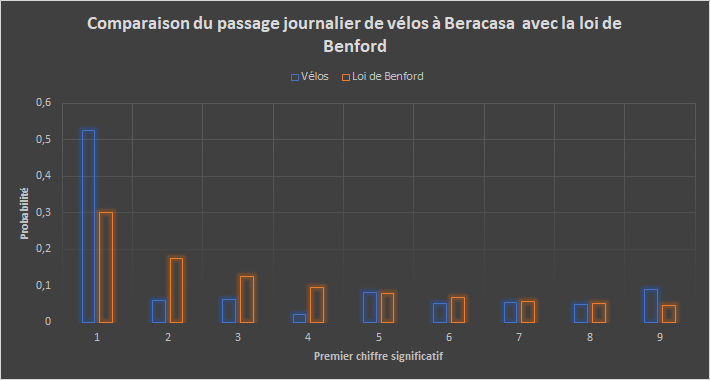
\includegraphics{Images/histogramme_velos.png}
\caption{Figure 5 : Histrogramme de la répartition du 1er chiffre
significatif du passage journalier de vélos en comparaison avec la loi
de Benford.}
\end{figure}

Dans ce cas la proportion du chiffre \(1\) est de plus de \(50 \%\)
contre \(30 \%\) pour la \textbf{loi de Newcomb-Benford}. La différence
de répartition des chiffres \(2, 3, 4, 5\) est aussi notable, elle est
même environ \(2\) fois moins élevée.\\
Visuellement, nous pourrions penser que la répartition de ces données ne
suit pas la \textbf{loi de Newcomb-Benford}. Il est courant de ne pas
retrouver la loi de Newcomb-Benford dans des données brutes commme
celles-ci, on la retrouve empiriquement plus souvent dans des données
dîtes de \textbf{deuxième génération} comme des sommes ou des produits.

\hypertarget{nombres-guxe9nuxe9ruxe9s-par-les-humains.}{%
\subsection{Nombres générés par les
humains.}\label{nombres-guxe9nuxe9ruxe9s-par-les-humains.}}

Après avoir observé ces quelques jeux de données, nous étions en mesure
de dire si ces données semblaient ou non suivre la loi de
Newcomb-Benford, le problème qui en découle est qu'une simple
observation n'est pas très fiable, difficile de prendre une décision sur
un constat visuel. En effet, se tromper dans l'interprétation peut
entrainer deux types d'erreur, la première étant de faussement déceler
une fraude (ce que nous appelerons \textbf{le risque de première
espèce}) et la deuxième de laisser passer une fraude. Ces erreurs ont un
coût pour l'institut qui essaye de les réprimer, celui d'engager des
démarches de détections approffondies inutiles ou de ne pas percevoir
les taxes dues dans le cas de la fraude fiscale par exemple.

Le but est donc de minimiser le coût que peuvent engendrer les erreurs
sus-mentionnées, pour se faire l'utilisation d'outils scientifiques est
de rigeur. Les outils que nous arboderons dans la suite sont les test
d'adéquations, ces tests servent à vérifier si un ensemble de nombre
suit ou non une loi de probabilité donnée (pour nous c'est la loi de
Newcomb-Benford).

TRANSITION AVEC LES TESTS Une inspection visuelle ne suffit pas, l'outil
pour ça c'est les tests d'adéquation à la loi de Benford erreur 1ere
espèce rejeter Ho (c'est dire que c'est pas benford alors que ca l'est,
dire qu'il y a fraude alors que non) erreur seconde espece (ne pas
rejeter H0 à tord, laisser passer une fraude) En stat l'erreur de 1ere
espèce est souvent plus présente On se dit pas qu'il y a fraude on
suspecte la fraude on lance une audit (ca coute des sous) dans tous les
cas on risque de faire une erreur (mettre le tableau)

\hypertarget{tests}{%
\section{Tests}\label{tests}}

PARLER DES TESTS DE MANIERE GENERALE, plutot theorique

le test privilégié est le test de chi2 quand c'est une problème qui a
une certaine importance pleins d'autres tests qui existent (package R
Benford test le seul test important dans ce package est celui du Chi2,
2ème package Benford smooth test créé par samuel et credo plus
spécifique au problème disponible sur le site CRAN) Les deuxièmes tests
sont mieux car plus puissantes, cad qu'ils détectent plus de fraudes. On
veut le test le plus puissant possible, a 5\% faire une description des
outils/tests

données fiscales sur plusieurs années de 20 régions italiennes, test de
chi2 (c'est pas un test très puissant, ne permet pas nécessairement de
détecter les fraudes.) Il ont mis que la statistique de test mais pas la
p-value

\hypertarget{application-des-tests}{%
\section{Application des tests}\label{application-des-tests}}

\hypertarget{application-a-des-donnuxe9es-fiscales-italiennes}{%
\subsection{Application a des données fiscales
italiennes}\label{application-a-des-donnuxe9es-fiscales-italiennes}}

\hypertarget{cas-covid}{%
\subsection{CAS COVID}\label{cas-covid}}

Un chinois a affirmé qu'il n'y avait pas eu fraudes en Chine

\hypertarget{bibliographie}{%
\section{Bibliographie}\label{bibliographie}}

\end{document}
